% !TeX TS-program = pdflatex
\documentclass{beamer}

\usepackage{tikz}
\setbeamercolor{background canvas}{bg=blue!30!black}
\setbeamertemplate{navigations symbols}{}
\usetikzlibrary{calc}
\def\xmin{-30}
\def\xmax{1.1\paperwidth}
\def\ymin{0}
\def\ymax{1.1\paperheight}


\begin{document}
\begin{frame}
\begin{tikzpicture}[remember picture, overlay]

\node at (current page.center) {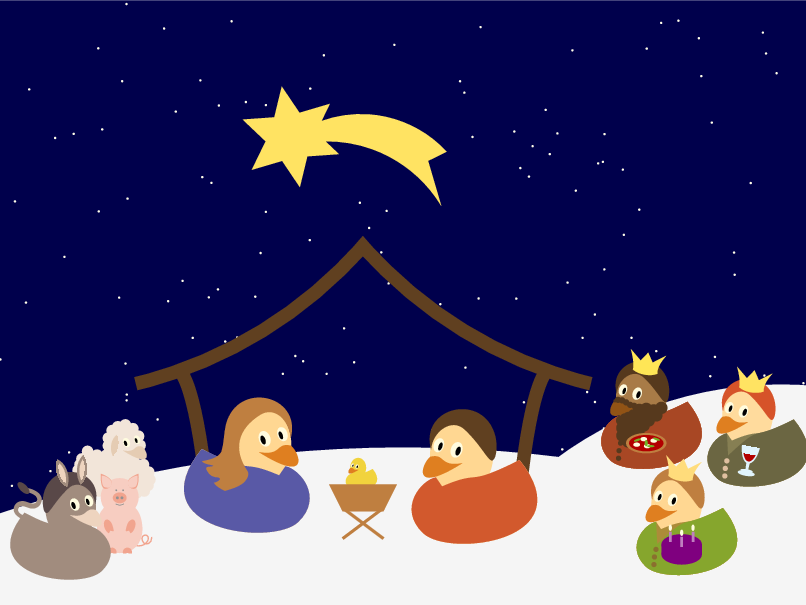
\includegraphics[width=\paperwidth]{NightDivine}};
\node<1-400>[xshift=200-0.5*\thepage] at (current page.center) {\includegraphics[width=\paperwidth]{Kings}};
\node<401-> at (current page.center) {\includegraphics[width=\paperwidth]{Kings}};
\node at ({5.4+0.1*sin(\thepage)},{28.8-0.0472*(\thepage)}) {
\includegraphics[width=\paperwidth]{snowflakes}};

\pause[500]
\end{tikzpicture}
\end{frame}
\end{document}